\documentclass[12pt, spanish]{beamer}
\usepackage[spanish]{babel}
\usepackage{caption}
\usepackage{minted}
\usepackage{listings}
\usepackage{multicol}
\usepackage{blindtext}
\usepackage{wrapfig}
\usepackage{hyperref}

\setlength{\columnseprule}{0.4pt}

\setlength{\columnsep}{0.1cm}
\usetheme{Madrid}

\title{\LaTeX es \textit{muy} sencillo de usar\ldots{}}
\author[CMA]{Carlos Miguel Alonso}
\institute{ACM UPM}
\date{\today}

\begin{document}

\begin{frame}
   \thispagestyle{empty}
   \titlepage
\end{frame}

\begin{frame}
    \centering
    {\Large \textbf{ENLACE}}
\end{frame}

\begin{frame}
    \centering
    \begin{alertblock}{Disclaimer}
        \LaTeX es \textbf{inmenso}, y no pretendo cubrir todo, solo lo que \textbf{yo} creo que es esencial/básico.\\
        Hay \textbf{muchísimos} comandos y paquetes para hacer cada cosa.\\
        Explorar es divertido :D 
    \end{alertblock}
\end{frame}

\begin{frame}{\LaTeX, que no látex}
    
    \begin{block}{¿Qué es?}
        Sistema de \textbf{composición de textos} orientado a la creación de documentos escritos de \textbf{alta calidad tipográfica}, cuyo uso mayoritario es la creación de \textbf{documentos científicos} (artículos y libros).

        \LaTeX{} es un software libre bajo la \textit{Latex Project Public License - LPPL}
    \end{block}
    \pause
    \hspace{2cm}


    \begin{block}{Bits de historia\ldots{}}
        \begin{itemize}
            \item Creado por Leslie Lamport en 1984 \ldots{}
            \pause
            \item es el sucesor de TeX creado por Donald Knuth en 1978 (*)
            \pause
            \item \textit{The \LaTeX{} Project} desarrollando \LaTeX{}3 
        \end{itemize}
    \end{block}
    
\end{frame}
\begin{frame}{¿Dónde empezar?}
    \begin{columns}
        \column{0.5\textwidth}

            \pause

            \begin{center}
                \textbf{\href{https://overleaf.com}{overleaf.com}}
            \end{center}
            \begin{itemize}
                \item[+] 0 cosas que instalar (out-of-the-box) 
                \item[+] De ``botón gordo''
                \item[+] Colaborativo
                \item[-] Requiere internet
                \item[-] ``Funciona''
            \end{itemize}

            \pause

        \column{0.5\textwidth}
            
            \begin{center}
                \textbf{en local}        
            \end{center}
            \begin{itemize}
                \item[+] No requiere internet
                \item[+] Editor y consola a tu gusto
                \item[-] Instalar \textbf{bastantes} paquetes
            \end{itemize}

    \end{columns}
\end{frame}
\begin{frame}{Comenzando el documento\ldots}

    \begin{block}{\textbackslash documentclass[\textit{ops}]\{\textit{type}\}}
        Define el tipo de documento y sus propiedades (más) básicas
    \end{block}

    \pause

    \vspace{0.5cm}

    \begin{columns}

        \column{0.5\textwidth}
        \textbf{Tipos de documentos}
        \begin{itemize}
            \item \textbf{article}
            \item \textbf{report}
            \item slides/\textbf{beamer}
            \item book
            \item letter
            \item \textit{clase propia}
        \end{itemize}
        
        \pause
        
        \column{0.5\textwidth}
        \textbf{Opciones del documento}
        \begin{itemize}
            \item font size (\textit{10pt}, 12pt, ...)
            \item page size
            \item \texttt{landscape}
            \item \texttt{draft}
            \item \texttt{twoside}
            \item y más\ldots{}
        \end{itemize}
        
    \end{columns}
    
\end{frame}



\begin{frame}{Comenzando el documento\ldots}

    \begin{block}{\textbackslash usepackage[\textit{ops}]\{\textit{pkg-name}\}}
        Sentencia para importar/referenciar paquetes
    \end{block}

    \pause
    \vspace{0.75cm}

    \begin{block}{\textbackslash begin\{document\} \ldots{} \textbackslash end\{document\}}
        Bloque \textit{document} que contiene todo el documento (ya sea en un solo archivo o en múltiples archivos).
    \end{block}

    \pause
    \vspace{0.5cm}

    \begin{center}
        \textit{¡Demo time!}
    \end{center}
\end{frame}
\begin{frame}{Portada}

    \begin{block}{\small {\texttt{\textbackslash title}\{\textit{text}\}, \texttt{\textbackslash date}\{\textit{text}\}, \texttt{\textbackslash author}\{\textit{text}\} y \texttt{\textbackslash maketitle}\{\}}}
    Especificamos \textit{título}, \textit{fecha} y \textit{autores}*, y luego en el cuerpo del documento, creamos el la portada antes que nada.
    \end{block}

    \pause
    
    \begin{columns}
        \column{0.5\textwidth}
            \hspace{1.5cm}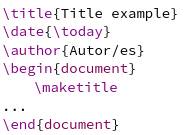
\includegraphics[width=0.5\textwidth]{images/make_title.png}
        \column{0.5\textwidth}
            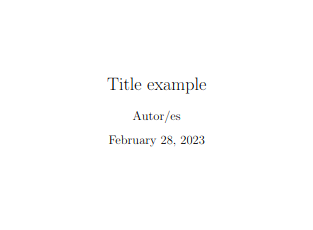
\includegraphics[width=\textwidth]{images/make_title_res.png}
    \end{columns}

    \pause

    \centering
    \textit{O podemos crear la portada mano\ldots{} \textleftarrow\: \textbf{Recomendable}}

\end{frame}
\begin{frame}{Capitulando}

    \begin{columns}
        \column{0.5\textwidth}
            \hspace{0.75cm}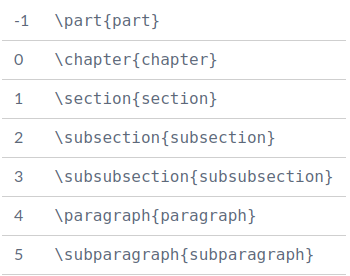
\includegraphics[width=0.75\textwidth]{images/sections.png}

        \column{0.5\textwidth}
            \begin{itemize}
                \item En artículos, lo más alto es la sección
                \item En \textit{report} y \textit{book}, lo más alto es \texttt{part} y \texttt{chapter} 
            \end{itemize}
    \end{columns}
    
    \vspace{0.5cm}
    \pause
    
    \begin{block}{}
    El comando \texttt{\textbackslash tableofcontents\{\}} crea el índice del documento (se puede poner en su propia página).\\
    \texttt{\textbackslash listoffigures\{\}} y \texttt{\textbackslash listoftables\{\}} hacen lo mismo con las figuras y tablas del documento\ldots{}
    \end{block}
    
\end{frame}
\begin{frame}{Dando formato\ldots{}}
    \centering
    \begin{tabular}{l l l}
        Formato & In-line & Bloque\\\hline
        \textbf{negrita} & \texttt{\textbackslash textbf\{text\}} & \texttt{\{\textbackslash textbf text\}}\\
        \textit{cursiva} & \texttt{\textbackslash textit\{text\}} & \texttt{\{\textbackslash textit text\}}\\
        \texttt{Typewriter} & \texttt{\textbackslash texttt\{text\}} & \texttt{\{\textbackslash texttt text\}}\\
        \textsc{mayus/minus} & \texttt{\textbackslash textsc\{text\}} & \texttt{\{\textbackslash textsc text\}}\\\hline \pause
        {\tiny Tiny} & & \texttt{\{\textbackslash tiny text\}}\\
        {\scriptsize Scriptsize} & & \texttt{\{\textbackslash scriptsize text\}}\\
        {\small Small} & & \texttt{\{\textbackslash small text\}}\\
        {\large large} & & \texttt{\{\textbackslash large text\}}\\
        {\Large Large} & & \texttt{\{\textbackslash Large text\}}\\
        {\Large LARGE} & & \texttt{\{\textbackslash LARGE text\}}\\
        {\huge huge} & & \texttt{\{\textbackslash huge text\}}\\
        {\Huge Huge} & & \texttt{\{\textbackslash Huge text\}}
    \end{tabular}
\end{frame}


\begin{frame}{Alienando el texto}{Saltar y espaciar}

    \begin{columns}
        \column{0.5\textwidth}
        \begin{itemize}
            \item \textbf{Saltos de línea}
            \begin{itemize}
                \item \texttt{\textbackslash\textbackslash}
                \item \texttt{\textbackslash newline}
                \item \texttt{\textbackslash hfill\textbackslash break}
            \end{itemize}

            \item \textbf{Saltos de página}
            \begin{itemize}
                \item \texttt{\textbackslash clearpage}
                \item \texttt{\textbackslash newpage}
            \end{itemize}
        \end{itemize}

        \pause
        
        \column{0.5\textwidth}
        \begin{itemize}
            \item \textbf{Espaciado horizontal}
            \begin{itemize}
                \item \texttt{\textbackslash hspace\{2cm\}}
                \item \texttt{\textbackslash hfill}
                \item \texttt{\textbackslash hrulefill}
                \item \texttt{\textbackslash dotfill}
            \end{itemize}
            
            \item \textbf{Espaciado vertical}
            \begin{itemize}
                \item \texttt{\textbackslash vspace\{2cm\}}
                \item \texttt{\textbackslash vfill}
                \item \texttt{\textbackslash smallskip}
                \item \texttt{\textbackslash medskip}
                \item \texttt{\textbackslash bigskip}
            \end{itemize}
        \end{itemize}
    \end{columns}
    
\end{frame}


\begin{frame}{Alienando el texto}{Márgenes}
    \centering
    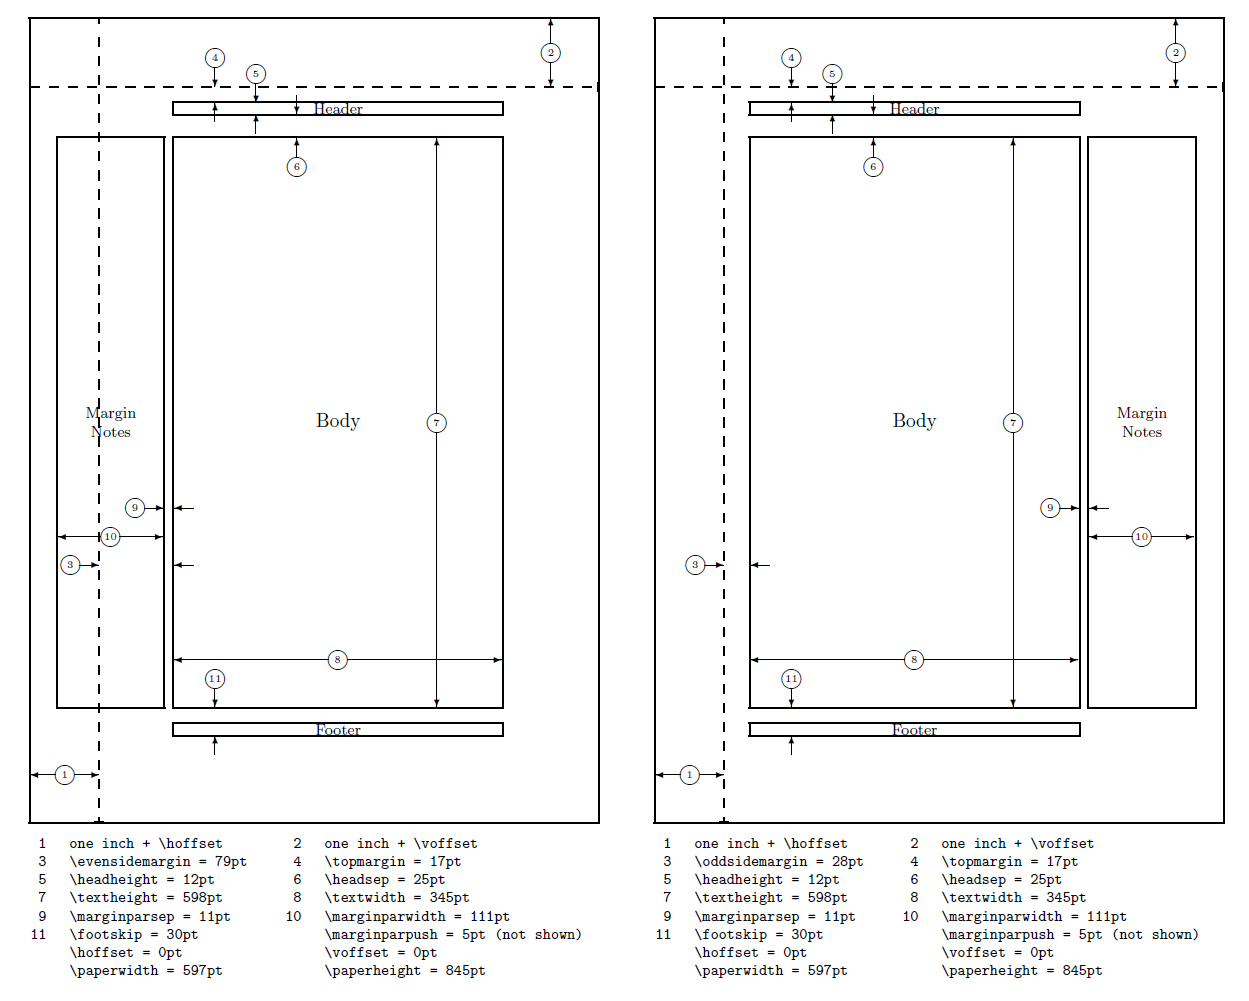
\includegraphics[width=0.75\textwidth]{images/layout.png}
\end{frame}

\begin{frame}{Alineando el texto}{Alineación de texto}
    \begin{columns}
        \column{0.5\textwidth}
            \begin{itemize}
                \item \textbf{Built-in}
                \begin{itemize}
                    \item \textbackslash raggedright
                    \item \textbackslash raggedleft
                    \item \textbackslash centering
                \end{itemize}
            \end{itemize}

        \pause
        
        \column{0.5\textwidth}
            \begin{itemize}
                \item \textbf{ragged2e}
                \begin{itemize}
                    \item \textbackslash Flush1Right
                    \item \textbackslash FlushLeft
                    \item \textbackslash Center
                    \item \textbackslash justify
                \end{itemize}
            \end{itemize}
    \end{columns}
\end{frame}
\begin{frame}[fragile]{Listas}
    \begin{columns}
        \column{0.5\textwidth}
            \centering
            \hspace{1cm}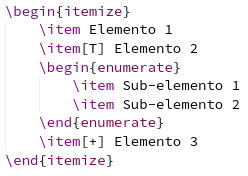
\includegraphics[width=0.75\textwidth]{images/list.png}

        \column{0.5\textwidth}
            \begin{itemize}
                \item Elemento 1
                \item[T] Elemento 2
                \begin{enumerate}
                    \item Sub-elemento 1
                    \item Sub-elemento 2
                \end{enumerate}
                \item[+] Elemento 3
            \end{itemize}
    \end{columns}
\end{frame}


\begin{frame}[fragile]{Tablas}

    \begin{center}
        
        \vspace{-1cm}\hspace{1cm}\begin{minted}{latex}
                \begin{tabular}{l|c r}
                    A & B & C \\\hline
                    D & E & F \\
                    G & H & I 
                \end{tabular}
        \end{minted}
    
        \vspace{1.5cm}
        
        \begin{tabular}{l|c r}
            A & B & C \\\hline
            D & E & F \\
            G & H & I 
        \end{tabular}

        \vspace{1cm}

        \textit{¡Demo time v2!}

    \end{center}

\end{frame}
\begin{frame}[fragile]{Columnas}
    \begin{columns}
        \hspace{1cm}\column{0.5\textwidth}
            Paquete \textbf{multicols}
            {\scriptsize
            \begin{minted}{latex}
\setlength{\columnseprule}{0.4pt}
...
\begin{multicols}{3}
    [
    Linea texto
    ]
Cuerpo de las columnas
\end{multicols}
            \end{minted}
            }

        \column{0.5\textwidth}
            \textbf{columns}
            {\scriptsize
            \begin{minted}{latex}
\begin{columns}
    \column{0.33\textwidth}
        Texto columna 1...
    \column{0.33\textwidth}
        Texto columna 2...
    \column{0.33\textwidth}
        Texto columna 3...
\end{columns}
            \end{minted}
            }
    \end{columns}
\end{frame}


\begin{frame}{Columnas}{Columnas de texto continuo\ldots{} (\texttt{multicol})}
    \begin{multicols}{3}
        [
        Linea que no se incluye en las columnas especificadas
        ]
        \blindtext
    \end{multicols}
\end{frame}


\begin{frame}[fragile]{Columnas}{Columnas manuales\ldots{} (\texttt{columns})}
    \begin{columns}
        \column{0.33\textwidth}
            Texto columna 1...
        \column{0.33\textwidth}
            Texto columna 2...
        \column{0.33\textwidth}
            Texto columna 3...
    \end{columns}
\end{frame}
\begin{frame}{Meter imágenes es sencillo\ldots{}}
    \begin{block}{\textbackslash \texttt{includegraphics[ops]\{img-path\}}}
    Mandato para incluir una imagen en el documento, siguiendo las opciones especificadas...
    
    \begin{itemize}
        \item \textbf{Opciones de una imagen} (ops)
        \begin{itemize}
            \item \texttt{scale}
            \item \texttt{width}
            \item \texttt{height}
            \item \texttt{angle}
        \end{itemize}
    \end{itemize}        
    
    \end{block}    

\end{frame}

\begin{frame}[fragile]{Meter imágenes es sencillo no?\ldots{} no?}

{\small
    \begin{minted}{latex}
        \graphicspath{ {images/} }
        ...
        \includegraphics[width=5cm]{frog.jpeg}
    \end{minted}
}
    \vspace{1cm}
    \pause
    \begin{center}
        \includegraphics[width=5cm]{images/frog.jpeg}
    \end{center}
\end{frame}


\begin{frame}[fragile]{Meter imágenes es sencillo no?\ldots{} no?}
    \begin{block}{\texttt{\textbackslash begin\{figure\}[ops]\ldots{} \textbackslash end\{figure\}}}
    Bloque que permite insertar una imagen con mayor control sobre el posicionamiento, así como añadir más información (captions y ref).    
    \end{block}
    \textbf{Opciones de posicionamiento} (se pueden combinar)
    \begin{itemize}
        \item \texttt{h}: donde el código (``here'')
        \item \texttt{t}: al inico de la página (``top'')
        \item \texttt{b}: al final de la página (``bottom'')
        \item \texttt{p}: en una nueva página (``page'')
        \item \texttt{!}: fuerza la posicion dada
        \item \texttt{H}: requiere pkg. \texttt{float}
    \end{itemize}
    
\end{frame}


\begin{frame}[fragile]{Meter imágenes es sencillo no?\ldots{} no?}

    {\small
    \begin{minted}{latex}
    \begin{figure}%[ h t b p ! H ]
        \centering
        \includegraphics[width=5cm]{frogs.jpeg}
        \caption{Frongus}
        \label{fig:frongus}
    \end{figure}
    \end{minted}
    }

    \pause
    
    \begin{figure}
        \centering
        \includegraphics[width=5cm]{images/frogs.jpeg}
        \caption{Frongus}
        \label{fig:frongus}
    \end{figure}
\end{frame}


\begin{frame}{Meter imágenes \textbf{bien} no es sencillo...}{Alrededor de texto (\texttt{wrapfig})}

    \pause
    % Del paquete (como no) wrapfig
    \begin{wrapfigure}{r}{0.5\textwidth}
        \begin{figure}
            \centering
            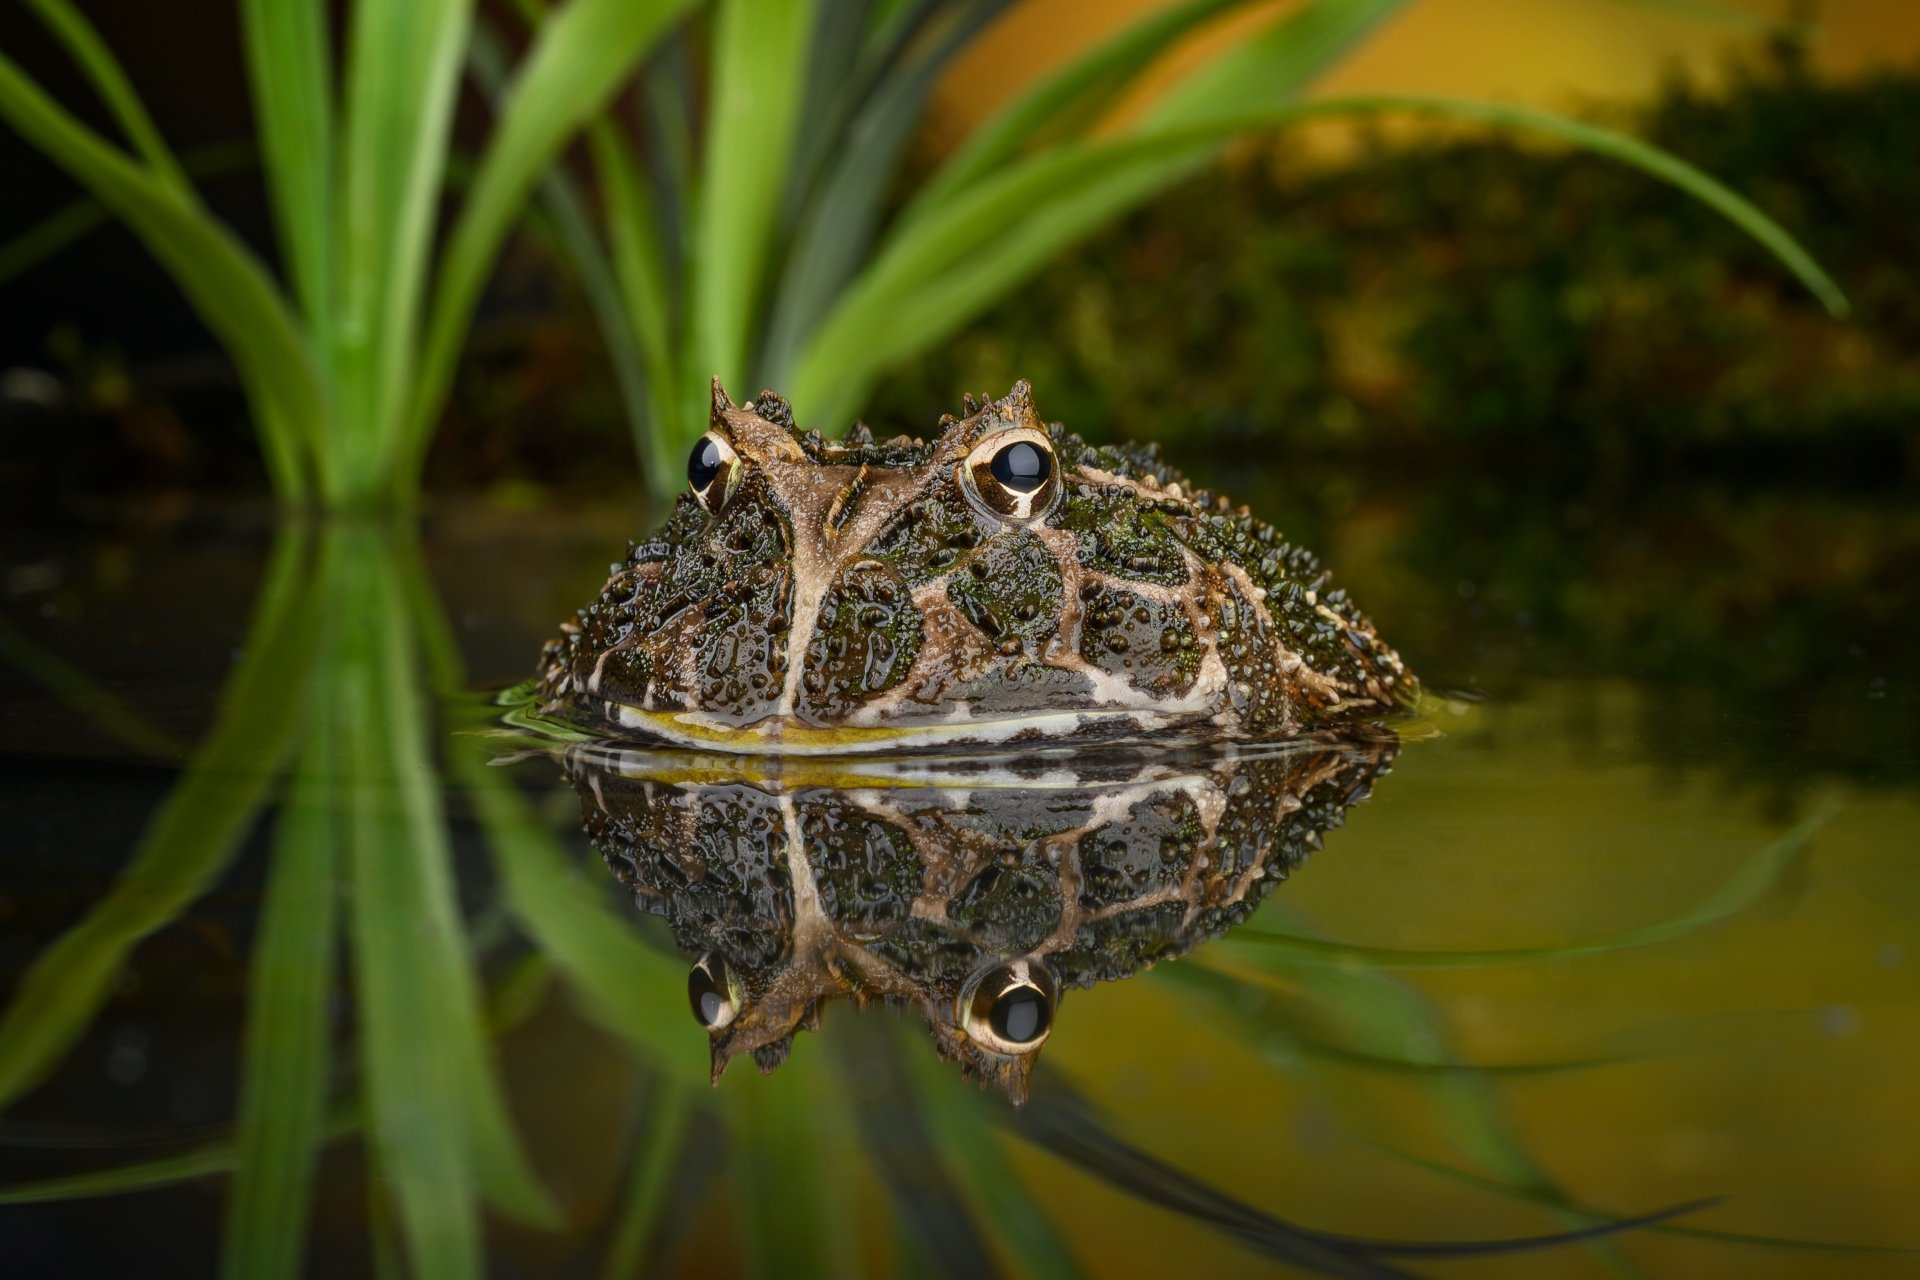
\includegraphics[width=5cm]{images/le_frog.jpeg}
            \caption{Le Frog}
            \label{fig:le_frog}
        \end{figure}
    \end{wrapfigure}
    Texto que habla de la Figura \ref{fig:le_frog}\ldots{}
    \blindtext
    
\end{frame}

\begin{frame}[fragile]{Meter imágenes \textbf{bien} NO es sencillo...}{Alrededor de texto (\texttt{wrapfig})}

{\small
\begin{minted}{latex}
    Texto...
    % r es right, pero
    % % r-R | l-L | i-I | o-O (mayus = float)
    \begin{wrapfigure}{r}{0.5\textwidth}
        \begin{figure}
            \centering
            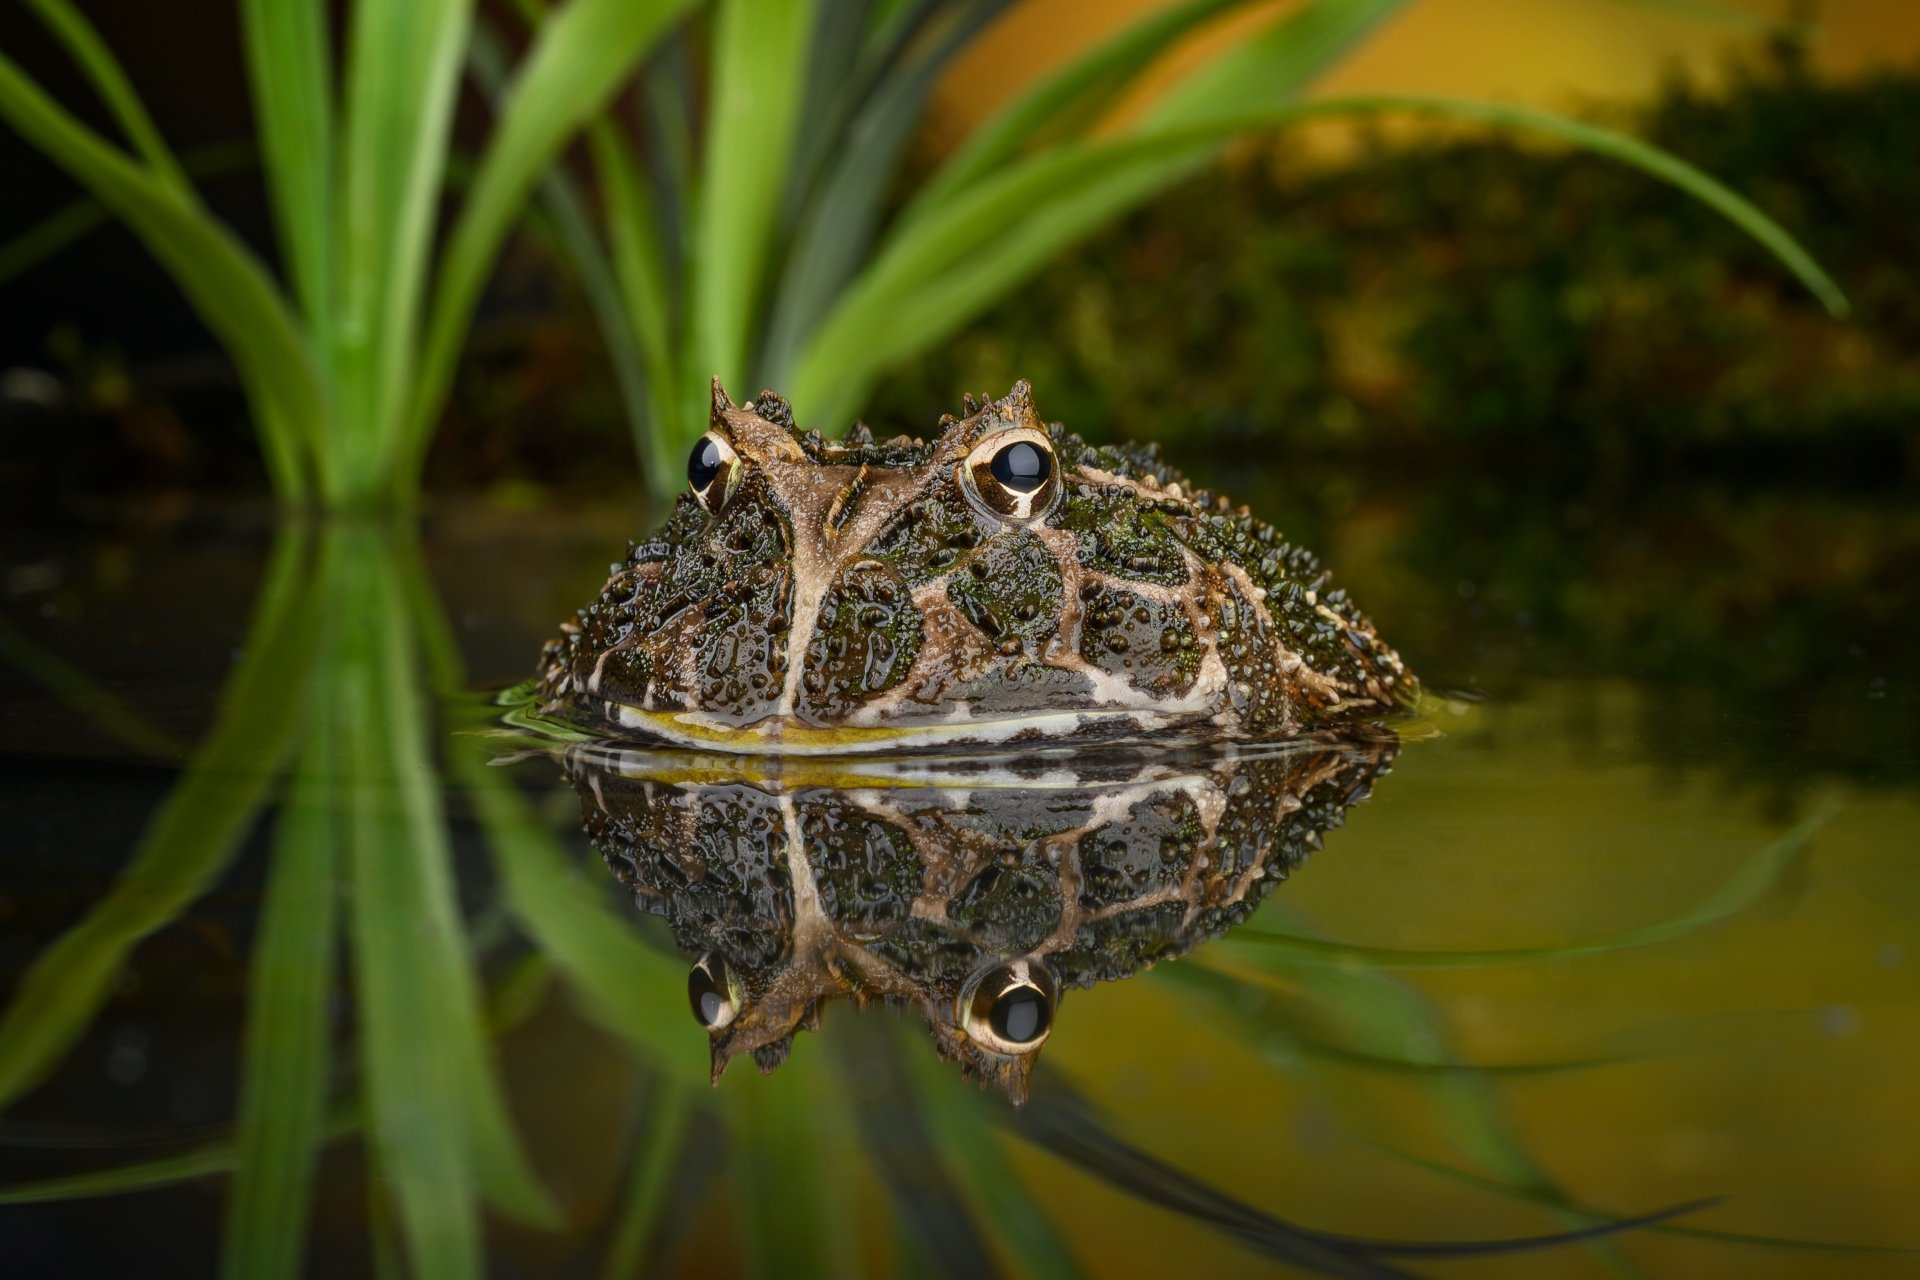
\includegraphics[width=5cm]{images/le_frog.jpeg}
            \caption{Le Frog}
            \label{fig:le_frog} % Genera ref para \ref
        \end{figure}
    \end{wrapfigure}
    Texto que habla de la Figura \ref{fig:le_frog}\ldots{}
    Más texto...
\end{minted}
}
    
\end{frame}


\begin{frame}{Lo de los números\ldots{} Matemáticas}
    
    \pause
    
    \begin{itemize}
        \item \textbf{In-Line} (parte del texto) $\Rightarrow$ $e^{\iota\pi}+1=0$
        \begin{itemize}
           \item \texttt{\textbackslash (\ldots{}\textbackslash )}
           \item \texttt{\$\ldots{}\$} 
           \item \texttt{\textbackslash begin\{math\}\ldots{}\textbackslash end\{math\}}
        \end{itemize}
    \vspace{0.5cm}
        \pause
        \item \textbf{Bloque} (apartadas del texto)
        \begin{itemize}
            \item \texttt{\textbackslash [\ldots{}\textbackslash]}
            \item \texttt{\textbackslash begin\{displaymath\}\ldots{}\textbackslash end\{displaymath\}}
            \item \texttt{\textbackslash begin \{equation\}\ldots{}\textbackslash end\{equation\}} (*)
        \end{itemize}
    \end{itemize}
    
    \vspace{0.5cm}

    \begin{columns}
        \column{0.5\textwidth}
            \begin{equation}
                \frac{n!}{k!(n-k)!} = \binom{n}{k}
            \end{equation}
    
        \column{0.5\textwidth}
            \begin{equation*}
                \int\limits_{-\infty}^{\infty}f(x)dx
            \end{equation*}
    \end{columns}
    

\end{frame}
\begin{frame}[fragile]{Mostrando código\ldots{}}{\texttt{verbatim}}

    \pause

    {\scriptsize
    \begin{minted}{latex}
\begin{verbatim}
Esta charla de \LaTeX{} se aloja en el Capítulo de Estudiantes de ACM de la UPM se
dedica a difundir el conocimiento informático: cursos, talleres, concursos, charlas...
\end{verbatim}
    \end{minted}
    }

    \vspace{1cm}
    \pause

    \begin{verbatim}
Esta charla de \LaTeX{} se aloja en el Capítulo de Estudiantes de ACM de la UPM se dedica a difundir el conocimiento informático: cursos, talleres, concursos, charlas...
    \end{verbatim}


\end{frame}


\begin{frame}[fragile]{Mostrando código\ldots{} Listings}{\texttt{lstlisting} del paquete \texttt{listings}}
    \begin{block}{}
    \texttt{\textbackslash begin[options]\{lstlisting\}\ldots{}\textbackslash end\{lstlisting\}}
    \end{block}

    \begin{lstlisting}[language=Python, caption=Python example]
def sum(val1, val2):
    return val1+val2
    \end{lstlisting}

{\small
    \begin{minted}{latex}
\begin{lstlisting}[language=Python, caption=Python example]
def sum(val1, val2):
    return val1+val2
\end{lstlisting}
    \end{minted}
}

\end{frame}


\begin{frame}{Mostrando código\ldots{} Listings}{\texttt{lstlisting} del paquete \texttt{listings}}
    \begin{block}{Definición de estilo propio}
        \texttt{\textbackslash lstdefinestyle\{mystyle\}\{\ldots{}\}}
        \texttt{\textbackslash lstset\{style=mystyle\}}
        \vspace{1.5cm}

        \textit{Listings tiene muchas opciones de personalización para mostrar el código como más guste al escritor}
    \end{block}

    \pause

    \centering
    \textit{¡Demo time 3: Back for more!}
\end{frame}
\begin{frame}{Recap de pequeñas cosas útiles}
    \begin{block}{Creando comandos}
        \texttt{\textbackslash newcommand\{\textbackslash nombre\}[N][M]\ldots{}\{\ldots{}\}}

        \begin{itemize}
            \item[-] \texttt{N}: número de argumentos
            \item[-] \texttt{[M]\ldots{}}\: Valores por defecto de los parámetros
            \item[-] Accediendo a los parámetros: \#X (X = número del parámetro)
        \end{itemize}
    \end{block}

    \pause
    
    \begin{block}{Enlaces con \texttt{hyperref}}
        \texttt{\textbackslash href\{url-mac-url.org\}\{FREE-BEER\}} $\Rightarrow$ \href{https://upm.acm.org/wp/}{ACMUPM}
    \end{block}

    \pause

    \begin{block}{Importando código \LaTeX{} de otro fichero}
        \texttt{\textbackslash include\{path-to-file.tex\}}
    \end{block}
    
\end{frame}


\begin{frame}{Y muuuuuucho más\ldots{}}
    \begin{itemize}
        \item Cabecera y pie de página del documento\pause
        \item Crear clases y paquetes propios\pause
        \item Diagramas (e.g. TikZ)\pause
        \item Presentaciones con \texttt{beamer} (¡como estas diapositivas!) 
        \item Ajedrez! (paquete \texttt{xskak})\pause
        \item y un larguísimo etc\ldots{}
    \end{itemize}
\end{frame}


\begin{frame}
    \centering
    Muchísimas gracias por escuchar mi sufrimiento :)
\end{frame}


\end{document}